\chapter{定态散射理论 (Stationary Scattering)}\label{ch:stationary}

\section{从时间相关到时间无关的描述}

在前面几章中我们建立了散射问题的\emph{时间相关}（time-dependent）的表述：
入射态 $|\psi_{\text{in}}\rangle$ 在 $t\to-\infty$ 时趋于一个自由波包 $U_0(t)|\phi\rangle$；
经过相互作用区域以后，在 $t\to+\infty$ 时又趋于另外一个自由波包 $U_0(t)|\phi'\rangle$。
两组渐近态之间的变换矩阵正是散射 $\Smat$ 矩阵：
\begin{equation}
  \Smat = \Omega_-^\dagger\,\Omega_+\,,
  \qquad
  |\phi\pm\rangle \equiv \Omega_\pm |\phi\rangle\,.
\end{equation}
其中 $\Omega_\pm$ 是 M\o ller 算符（见第~\ref{ch:Smat1P}~章），它把可归一化的自由
渐近态 $|\phi\rangle$ 映成 $t=0$ 时刻真实的散射态 $|\phi\pm\rangle$。

入射波包和出射波包都可以用自由的能量本征态 $|\vec p\rangle$ 叠加得到：
\begin{equation}
  |\phi\rangle = \int \rmd^3 p\, \phi(\vec p)\,|\vec p\rangle\,,
\end{equation}
那么自然就提示我们对每一个动量本征态 $|\vec p\rangle$ 单独定义一个对应的``散射态''，
这便是\emph{定态散射态}（stationary scattering state）：
\begin{equation}
  \boxed{\;|\vec p\pm\rangle \;\equiv\; \Omega_\pm |\vec p\rangle\;.\;}
  \label{eq:def-ppm}
\end{equation}

由于 $|\vec p\rangle$ 不是可归一化的态，$|\vec p\pm\rangle$ 同样是 $\Hmat$ 的
\emph{improper} 本征矢，不具有有限的 norm。但它们可以作为完备的展开基，把任何
真实的散射态展开为它们的叠加。这就是所谓的\emph{时间无关的表述}：把全部散射信息
凝缩到一组能量本征态 $|\vec p\pm\rangle$ 当中，不再需要显式地考虑波包的时间演化。

历史上人们最早就是用时间无关的描述来处理散射问题。对球对称势散射，可以证明
（这正是本章要建立的渐近形式）
\begin{equation}
  \psi_+(\vec x) \;=\; \langle \vec x|\vec p+\rangle
  \;\xrightarrow{r\to\infty}\;
  (2\pi)^{-3/2}\!\left[\,\rme^{\rmi\vec p\cdot\vec x}
  + f(\theta,\varphi)\,\frac{\rme^{\rmi p r}}{r}\right].
  \label{eq:stationary-asymp-intro}
\end{equation}
通常的量子力学教材就是从这一渐近边界条件出发求解定态薛定谔方程，本章我们要把它
跟前几章建立的算符语言衔接起来。

求解 $|\vec p\pm\rangle$ 通常有两种途径：
\begin{itemize}
  \item \textbf{积分方程}：跟 Green 算符 $G(z)$、$\Tmat(z)$ 满足的 Lippmann--Schwinger
        方程相联系；
  \item \textbf{微分方程}：直接求解定态薛定谔方程 $\Hmat|\vec p\pm\rangle =
        E_p|\vec p\pm\rangle$，并加上适当的渐近边界条件。
\end{itemize}

\begin{remark}
后面用到的约定：$\hbar=1$（在最后给出 $f$ 与 $T$ 矩阵元的关系时再恢复 $\hbar$，
方便和教科书对照）；$E_p = \vec p^{\,2}/(2m)$；$|\vec p\rangle$ 取
$\langle \vec x|\vec p\rangle = (2\pi)^{-3/2}\rme^{\rmi\vec p\cdot\vec x}$，
$\inn{\vec p'}{\vec p} = \delta^3(\vec p'-\vec p)$。
\end{remark}

\section{$|\vec p\pm\rangle$ 的基本性质}

\subsection{是 $\Hmat$ 的本征态}

$|\vec p\rangle$ 是自由 Hamiltonian $\Hmat_0$ 的本征态，$\Hmat_0|\vec p\rangle =
E_p|\vec p\rangle$。利用 M\o ller 算符的 intertwining 关系
\begin{equation}
  \Hmat\,\Omega_\pm \;=\; \Omega_\pm\,\Hmat_0\,,
  \label{eq:intertwining}
\end{equation}
立刻得到
\begin{equation}
  \Hmat|\vec p\pm\rangle
  = \Hmat\Omega_\pm|\vec p\rangle
  = \Omega_\pm \Hmat_0|\vec p\rangle
  = E_p\,\Omega_\pm|\vec p\rangle
  = E_p\,|\vec p\pm\rangle\,.
  \label{eq:H-eigenppm}
\end{equation}
即 $|\vec p\pm\rangle$ 是真实 Hamiltonian $\Hmat$ 的 improper 本征态，本征值
$E_p = \vec p^{\,2}/(2m)$ 跟自由渐近态 $|\vec p\rangle$ 完全一致。

\subsection{时间演化与 $t\to\mp\infty$ 渐近行为}

由于 $|\vec p\pm\rangle$ 是 $\Hmat$ 的本征态，
\begin{equation}
  U(t)|\vec p\pm\rangle \;=\; \rme^{-\rmi E_p t}|\vec p\pm\rangle\,,
  \qquad
  U_0(t)|\vec p\rangle \;=\; \rme^{-\rmi E_p t}|\vec p\rangle\,.
\end{equation}
注意它们随时间只是带一个总相位 $\rme^{-\rmi E_p t}$ ——所以从单个 $|\vec p\pm\rangle$
本身\emph{看不出}它在 $t\to\mp\infty$ 时趋于自由的 $|\vec p\rangle$！这正是
$|\vec p\pm\rangle$ 不是物理的可归一化态导致的``失真''。

要恢复时间相关的描述，必须做\emph{波包平滑（smearing）}。对一可归一化的 $\phi$，
$|\phi\pm\rangle = \int\!\rmd^3p\,\phi(\vec p)\,|\vec p\pm\rangle$，那么
\begin{equation}
  U(t)|\phi\pm\rangle
  = \int\!\rmd^3p\,\phi(\vec p)\,U(t)|\vec p\pm\rangle
  \;\xrightarrow{t\to\mp\infty}\;
  \int\!\rmd^3p\,\phi(\vec p)\,U_0(t)|\vec p\rangle
  = U_0(t)|\phi\rangle\,,
\end{equation}
回到了 M\o ller 算符的定义关系 $\lim_{t\to\mp\infty}U_0(-t)U(t)|\phi\pm\rangle =
|\phi\rangle$。在 smear 过的意义下我们也可以说：``入射（出射）渐近态
$|\vec p\rangle$ 对应的散射态在 $t=0$ 时刻是 $|\vec p+\rangle$（$|\vec p-\rangle$）''。

\subsection{完备性与正交归一}

由于 $\Omega_\pm$ 把 $\Hilb_{\text{free}}$ 等距映到 $\Hilb$ 中渐近完备的子空间
$\mathcal{R}=\Ran(\Omega_\pm)$，且 $\Omega_\pm^\dagger\Omega_\pm = \mathbf{1}$，
所以 $\{|\vec p\pm\rangle\}$ 在 $\mathcal{R}$ 上是正交完备的：
\begin{equation}
  \inn{\vec p'\pm}{\vec p\pm}
  = \matel{\vec p'}{\Omega_\pm^\dagger\Omega_\pm}{\vec p}
  = \delta^3(\vec p'-\vec p)\,.
  \label{eq:ppm-ortho}
\end{equation}

由渐近完备性 $\Hilb = \mathcal{R}\oplus\mathcal{B}$，其中 $\mathcal{B}$ 是束缚态张
成的子空间，所以 $\{|\vec p+\rangle\}\cup\{|n\rangle_{\text{bound}}\}$（同样
$\{|\vec p-\rangle\}\cup\{|n\rangle\}$）构成 $\Hilb$ 的一组完备基矢：
\begin{align}
  \mathbf{1}
  &= \int\!\rmd^3p\,|\vec p\rangle\langle\vec p|
   = \int\!\rmd^3p\,|\vec p+\rangle\langle\vec p+|+\sum_n |n\rangle\langle n|\nonumber\\
  &= \int\!\rmd^3p\,|\vec p-\rangle\langle\vec p-|+\sum_n |n\rangle\langle n|\,.
  \label{eq:completeness}
\end{align}
注意 $|\vec p+\rangle$ 和 $|\vec p-\rangle$ 都是同一个 $\Hmat$ 在同一本征值
$E_p$ 上的本征矢，意味着实际的能量本征空间是\emph{高度简并}的（既有 ``in'' 标记，
也有 ``out'' 标记，简并的方向数对应 $4\pi$ 立体角）。

\section{定态散射态满足的积分方程}

\subsection{用 $G$ 写的 Lippmann--Schwinger 方程}

第~\ref{ch:green}~章已经导出，对可归一化的态 $|\phi\rangle$，
\begin{equation}
  |\phi\pm\rangle \;=\; |\phi\rangle + \int\!\rmd^3 p\,
  G(E_p\pm \rmi\epsilon)\,\Vmat\,|\vec p\rangle\,\langle \vec p|\phi\rangle\,.
  \label{eq:LS-phipm}
\end{equation}
左右两边把 $|\phi\pm\rangle$ 和 $|\phi\rangle$ 用 $|\vec p\pm\rangle$、
$|\vec p\rangle$ 展开，$|\phi\rangle = \int\rmd^3 p\,\phi(\vec p)|\vec p\rangle$，
$|\phi\pm\rangle = \int\rmd^3 p\,\phi(\vec p)|\vec p\pm\rangle$，则
\begin{equation}
  \int\!\rmd^3 p\,\phi(\vec p)\,|\vec p\pm\rangle
  = \int\!\rmd^3 p\,\phi(\vec p)\Big(|\vec p\rangle
    + G(E_p\pm \rmi\epsilon)\,\Vmat\,|\vec p\rangle\Big)\,.
\end{equation}
由于这对任意 $\phi(\vec p)$ 都成立，被积函数必须相等，于是
\begin{equation}
  \boxed{\;|\vec p\pm\rangle \;=\; |\vec p\rangle
  + G(E_p\pm \rmi\epsilon)\,\Vmat\,|\vec p\rangle\;.\;}
  \label{eq:LS-G-ch09}
\end{equation}
这是定态散射态的 Lippmann--Schwinger 方程的第一种形式。$\pm \rmi\epsilon$ 处方
分别选取了出射（incoming wave at infinity is plane wave only, plus outgoing
spherical wave）和入射（plus incoming spherical wave）边界条件。

\subsection{用 $G_0$ 写的 Lippmann--Schwinger 方程}

利用 $GV = G_0 T$（见第~\ref{ch:green}~章），\eqref{eq:LS-G-ch09} 可以等价地用
自由 Green 算符 $G_0$ 写出：
\begin{equation}
  \boxed{\;|\vec p\pm\rangle \;=\; |\vec p\rangle
  + G_0(E_p\pm \rmi\epsilon)\,\Vmat\,|\vec p\pm\rangle\;.\;}
  \label{eq:LS-G0}
\end{equation}
这就是大多数教科书写下的 \emph{Lippmann--Schwinger 方程}。它是 $|\vec p\pm\rangle$
的隐式积分方程，可迭代得到 Born 级数：
\begin{equation}
  |\vec p+\rangle = |\vec p\rangle + G_0(E_p+\rmi 0)\Vmat|\vec p\rangle
  + G_0(E_p+\rmi 0)\Vmat G_0(E_p+\rmi 0)\Vmat|\vec p\rangle + \cdots\,.
  \label{eq:Born-state}
\end{equation}
此时我们手中已经有三个相互等价的 Lippmann--Schwinger 方程：
\begin{align}
  (1-G_0\Vmat)\,G &= G_0\,,\label{eq:LS-G-ch09-op}\\
  (1-\Vmat G_0)\,T &= \Vmat\,,\label{eq:LS-T-ch09}\\
  (1-G_0\Vmat)\,|\vec p\pm\rangle &= |\vec p\rangle\,.\label{eq:LS-state-op}
\end{align}

\subsection{壳上 $T$-矩阵元}

把 $T(z) = \Vmat + \Vmat G(z)\Vmat$ 作用到 $|\vec p\rangle$ 上：
\begin{equation}
  T(E_p\pm \rmi 0)|\vec p\rangle
  = \big[\Vmat + \Vmat G(\pm)\Vmat\big]|\vec p\rangle
  = \Vmat\big[\,\mathbf{1}+G(\pm)\Vmat\,\big]|\vec p\rangle
  = \Vmat\,|\vec p\pm\rangle\,.
  \label{eq:T-on-p}
\end{equation}
取左矢 $\langle\vec p'|$ 得到
\begin{equation}
  \boxed{\;t(\vec p'\leftarrow \vec p) \;\equiv\; \langle\vec p'|T(E_p+\rmi 0)|\vec p\rangle
  \;=\; \langle\vec p'|\Vmat|\vec p+\rangle\;.\;}
  \label{eq:t-onshell-1}
\end{equation}
这就是我们在前面章节频繁使用的\emph{在壳} $T$-矩阵元（``on-shell''指 $|\vec p|=
|\vec p'|$，但 $T$ 中能量参数取在 $E_p+\rmi 0$，与初态动能匹配）。

利用 $T(z)^\dagger = T(z^*)$，
\begin{equation}
  \langle\vec p'|T(E_{p'}+\rmi 0) = \langle\vec p' -|\Vmat
  \;\;\Longrightarrow\;\;
  t(\vec p'\leftarrow \vec p) = \langle\vec p'-|\Vmat|\vec p\rangle\,.
  \label{eq:t-onshell-2}
\end{equation}
两种写法在壳（$E_{p'}=E_p$）时一致。配合 \eqref{eq:Born-state} 立刻有
\begin{equation}
  t(\vec p'\leftarrow \vec p)
  = \langle\vec p'|\Vmat|\vec p\rangle
  + \langle\vec p'|\Vmat G_0\Vmat|\vec p\rangle + \cdots\,,
\end{equation}
即 $T$-矩阵元的 Born 展开。

\section{坐标表象的定态波函数}

\subsection{积分方程}

把 \eqref{eq:LS-G0} 投影到坐标 $\langle\vec x|$，并在中间插入完备性
$\int\rmd^3 x'\,|\vec x'\rangle\langle\vec x'|$：
\begin{equation}
  \langle\vec x|\vec p\pm\rangle
  = \langle\vec x|\vec p\rangle
  + \int\!\rmd^3 x'\,\langle\vec x|G_0(E_p\pm\rmi\epsilon)|\vec x'\rangle\,
    V(\vec x')\,\langle\vec x'|\vec p\pm\rangle\,.
  \label{eq:LS-coord}
\end{equation}
（这里假设 $V$ 在坐标表象是局域的：$\langle\vec x|\Vmat|\vec x'\rangle =
V(\vec x)\,\delta^3(\vec x-\vec x')$。）这就是教科书上熟悉的、关于波函数
$\psi^\pm(\vec x) \equiv \langle\vec x|\vec p\pm\rangle$ 的积分方程。

\subsection{自由 Green 函数 $\langle\vec x|G_0(z)|\vec x'\rangle$}

需要 $G_0(z)$ 的坐标表象。利用动量基插入完备性，
\begin{align}
  \langle\vec x|G_0(z)|\vec x'\rangle
  &= \int\!\rmd^3 p\,\frac{\langle\vec x|\vec p\rangle\langle\vec p|\vec x'\rangle}{z-E_p}
   = \frac{1}{(2\pi)^3}\int\!\rmd^3 p\,
     \frac{\rme^{\rmi \vec p\cdot(\vec x-\vec x')}}{z-\vec p^{\,2}/(2m)}\nonumber\\
  &= \frac{1}{(2\pi)^3}\int_0^\infty\! p^2\rmd p\int\rmd\Omega_p\,
     \frac{\rme^{\rmi p|\vec x-\vec x'|\cos\theta}}{z-p^2/(2m)}\nonumber\\
  &= \frac{-\rmi}{4\pi^2|\vec x-\vec x'|}\int_0^\infty p\,\rmd p\,
     \frac{\rme^{\rmi p|\vec x-\vec x'|}-\rme^{-\rmi p|\vec x-\vec x'|}}{z-p^2/(2m)}\nonumber\\
  &= \frac{\rmi m}{4\pi^2|\vec x-\vec x'|}\int_{-\infty}^{\infty}\rmd p\,
     \frac{p\,\rme^{\rmi p|\vec x-\vec x'|}}{p^2-2mz}\,.
\end{align}
对最后一行作 $p$-平面回路（沿上半平面闭合）求复变积分。$z$ 上方有一对极点
$p=\pm(2mz)^{1/2}$；按照 $\Im (2mz)^{1/2}>0$ 选取根号支，则上半平面上的极点是
$p_+ = +(2mz)^{1/2}$。由留数定理得
\begin{equation}
  \langle\vec x|G_0(z)|\vec x'\rangle
  = -\frac{m}{2\pi}\,\frac{\exp\!\big[\rmi(2mz)^{1/2}|\vec x-\vec x'|\big]}{|\vec x-\vec x'|}\,,
  \qquad \Im(2mz)^{1/2}>0\,.
  \label{eq:G0-coord}
\end{equation}

把 $z = E_p\pm\rmi 0$ 代入。由 $E_p = p^2/(2m)$，$(2mz)^{1/2}\to \pm p+\rmi 0$
（注意 $-$ 号选 ``$+\rmi 0$'' 时根号支变 $-p+\rmi 0$，同样保证 $\Im>0$）。所以
\begin{equation}
  \langle\vec x|G_0(E_p\pm\rmi 0)|\vec x'\rangle
  = -\frac{m}{2\pi}\,\frac{\rme^{\pm \rmi p|\vec x-\vec x'|}}{|\vec x-\vec x'|}\,.
  \label{eq:G0-eps}
\end{equation}
代回 \eqref{eq:LS-coord}，
\begin{equation}
  \langle\vec x|\vec p\pm\rangle
  = \langle\vec x|\vec p\rangle
  - \frac{m}{2\pi}\int\!\rmd^3 x'\,
    \frac{\rme^{\pm \rmi p|\vec x-\vec x'|}}{|\vec x-\vec x'|}\,V(\vec x')\,
    \langle\vec x'|\vec p\pm\rangle\,.
  \label{eq:LS-coord-explicit}
\end{equation}
\eqref{eq:LS-coord-explicit} 就是定态波函数 $\psi^\pm(\vec x)$ 满足的具体积分
方程。$+$ 号对应 \emph{outgoing}（出射球面波）边界，$-$ 号对应 \emph{incoming}
（入射球面波）边界。

\begin{remark}
回路选择的物理含义：$\rme^{+\rmi p|\vec x-\vec x'|}$ 跟 $\rme^{-\rmi E_p t}$ 配
合得到 $\rme^{\rmi(pr-E_p t)}$，这是\emph{向外}（指向 $\vec x$ 远离 $\vec x'$ 方
向）传播的球面波；反之 $-$ 号给出向内传播的球面波。这与下一节渐近形式的物理含义
完全一致。
\end{remark}

\subsection{大 $r$ 渐近形式与散射振幅}

假设势是有限程的：$V(\vec r)=0$ 当 $r>a$。考察大 $r$（$r\to\infty$、$r\gg a$）
区域的 $\langle\vec x|\vec p\pm\rangle$：积分中 $r'\le a$，因此可以做远场展开
\begin{equation}
  |\vec x-\vec x'| = \big(r^2 - 2\vec x\cdot\vec x' + r'^2\big)^{1/2}
  = r\Big[1 - \frac{\vec x\cdot\vec x'}{r^2} + O\!\Big(\frac{r'}{r}\Big)^2\Big]
  = r - \hat{\vec x}\cdot\vec x' + O\!\Big(\frac{r'^{\,2}}{r}\Big)\,,
\end{equation}
其中 $\hat{\vec x}=\vec x/r$。代入 \eqref{eq:LS-coord-explicit}，
\begin{equation}
  \langle\vec x|\vec p\pm\rangle
  = \langle\vec x|\vec p\rangle
  - \frac{m\,\rme^{\pm \rmi p r}}{2\pi r}\int\!\rmd^3 x'\,
    \rme^{\mp \rmi p\hat{\vec x}\cdot\vec x'}\,V(\vec x')\,
    \langle\vec x'|\vec p\pm\rangle
    \!\left[1+O\!\Big(\frac{a}{r}\Big)+O\!\Big(\frac{p a^2}{r}\Big)\right]\!.
\end{equation}
注意被积分的部分恰好是 \eqref{eq:t-onshell-2} 的逆：定义出射/入射方向的动量
$\vec p'\equiv \pm p\hat{\vec x}$（$+$对$+$，$-$对$-$），则
\begin{equation}
  \int\!\rmd^3 x'\,\rme^{\mp \rmi p\hat{\vec x}\cdot\vec x'}V(\vec x')
  \langle\vec x'|\vec p\pm\rangle
  = (2\pi)^{3/2}\,\langle \pm p\hat{\vec x}|\Vmat|\vec p\pm\rangle
  = (2\pi)^{3/2}\,t(\pm p\hat{\vec x}\leftarrow \vec p)\,.
\end{equation}
因此
\begin{equation}
  \langle\vec x|\vec p\pm\rangle
  \;\xrightarrow{r\to\infty}\;
  (2\pi)^{-3/2}\!\left[\rme^{\rmi\vec p\cdot\vec x}
  \;-\;(2\pi)^2 m\,\langle \pm p\hat{\vec x}|\Vmat|\vec p\pm\rangle\,
  \frac{\rme^{\pm\rmi p r}}{r}\right]\!.
  \label{eq:asymp-derived}
\end{equation}
与教科书中标准的渐近边界条件
\begin{equation}
  \psi^\pm(\vec x)\;\xrightarrow{r\to\infty}\;
  (2\pi)^{-3/2}\!\left[\rme^{\rmi\vec p\cdot\vec x}
  + f(p\hat{\vec x}\leftarrow\vec p)\,\frac{\rme^{\pm\rmi p r}}{r}\right]
  \label{eq:asymp-textbook}
\end{equation}
对比，立得
\begin{empheq}[box=\fbox]{equation}
  f(\vec k'\leftarrow \vec k) \;=\; -\,(2\pi)^2 m\,\langle\vec k'|\Vmat|\vec k+\rangle
  \;=\; -\,(2\pi)^2 m\,\langle\vec k'|T(E_k+\rmi 0)|\vec k\rangle\,.
  \label{eq:f-T-relation}
\end{empheq}
这正是\emph{从定态图像直接定义散射振幅与 $T$-矩阵元的关系}。在恢复 $\hbar$ 后
（$\vec p\to\hbar\vec k$，$\rmd^3p\to\hbar^3\rmd^3k$，$E=\hbar^2 k^2/(2m)$），上式
按通常的写法就是
\begin{equation}
  \boxed{\;f(\vec k'\leftarrow \vec k)
  \;=\; -\,\frac{(2\pi)^2 m}{\hbar^2}\,\langle\vec k'|\Tmat|\vec k\rangle\,.\;}
  \label{eq:f-T-hbar}
\end{equation}

\eqref{eq:asymp-derived}--\eqref{eq:f-T-relation} 同时实现了三件事情：
\begin{enumerate}
  \item 重新导出了教科书的渐近边界条件 \eqref{eq:asymp-textbook}，确认
        $\langle\vec x|\vec p\pm\rangle$ 在大 $r$ 处确实是``平面波 + 出射/入射
        球面波''；
  \item 把渐近振幅 $f$ 与算符语言下的在壳 $T$-矩阵元 $\langle\vec k'|T|\vec k\rangle$
        显式联系起来；
  \item 完成了\emph{时间相关}与\emph{时间无关}两种散射表述的等价性证明。
\end{enumerate}

\subsection{物理解读}

\eqref{eq:asymp-textbook} 中的两个解 $\psi^+$、$\psi^-$ 物理含义清晰：
\begin{itemize}
  \item $\psi^+ = \langle\vec x|\vec p+\rangle$：``in'' 态——平面波入射，加上一个
        \emph{出射}的球面波 $f\,\rme^{\rmi p r}/r$。这正是真实散射实验所对应的
        定态散射波函数。
  \item $\psi^- = \langle\vec x|\vec p-\rangle$：``out'' 态——平面波加上一个
        \emph{入射}的球面波 $f^{(-)}\,\rme^{-\rmi pr}/r$。在 LSZ 类型的论证（散射
        振幅的对偶表达）中会用到。
\end{itemize}

\section{时间无关表述：常见教科书做法}

许多量子力学教材的``正统''顺序是：
\begin{enumerate}
  \item \textbf{设 ansatz}：在无穷远处定态波函数取
        \eqref{eq:asymp-textbook} 的边界条件，从中读出散射振幅 $f$；
  \item \textbf{物理诠释}：平面波代表入射粒子流，球面波代表散射出去的粒子；用入
        射流密度归一，出射粒子单位时间单位立体角的数目除以入射通量给出微分散射
        截面
        \begin{equation}
          \frac{\rmd\sigma}{\rmd\Omega} = |f(\theta,\varphi)|^2\,;
          \label{eq:dsig-dOmega}
        \end{equation}
  \item \textbf{解方程}：把带有渐近边界条件的定态薛定谔方程 $(\Hmat-E_p)\psi=0$
        化为 \eqref{eq:LS-coord-explicit} 形式的积分方程，再化为 Lippmann--
        Schwinger 算符方程 \eqref{eq:LS-G0}，最终得到
        \begin{equation}
          f(\vec k'\leftarrow\vec k) = -(2\pi)^2 m\,\langle\vec k'|\Vmat|\vec k+\rangle\,;
        \end{equation}
        迭代求解再得到 Born 级数。
\end{enumerate}

我们前面的处理顺序则是反过来的：先有时间相关 + M\o ller 算符的语言，再定义
$|\vec p\pm\rangle$，最后从大 $r$ 渐近导出 \eqref{eq:asymp-textbook}。两条路径
在物理与数学上完全等价。

\begin{remark}[关于 $|\vec p\pm\rangle$ 的非物理性]
$|\vec p\pm\rangle$ 没有有限的 norm，不是物理可实现的态，是 $\Hmat$ 的 improper
本征态——这跟自由情形 $|\vec p\rangle$ 的地位完全相同。它们的作用是\emph{展开
基}：真实可归一的散射态在 $t=0$ 处可写成
\begin{equation}
  |\psi\rangle = |\phi+\rangle = \int\!\rmd^3p\,\phi(\vec p)\,|\vec p+\rangle\,,
  \qquad
  |\psi_{\text{in}}\rangle = \int\!\rmd^3p\,\phi(\vec p)\,|\vec p\rangle\,,
\end{equation}
两组展开系数 $\phi(\vec p)$ \emph{完全相同}。当 $\phi(\vec p)$ 集中在某一 $\vec
p_0$ 附近的极窄动量区间时，$\psi_{\text{in}}$ 趋近于一个准单色平面波，散射态的
物理性质就由 $|\vec p_0+\rangle$ 这一个本征态完全给出。
\end{remark}

\section{用波包恢复散射的坐标空间描述}

之前算微分散射截面是在动量空间中数 $\rmd\Omega$ 立体角内出射的粒子数
$N_{\text{sc}}(\rmd\Omega)$；为了把 \eqref{eq:dsig-dOmega} 跟实验中粒子计数器在
空间某方向上探测到的粒子数直接联系起来，需要在坐标空间中重新论证一遍。这里要结合
\eqref{eq:asymp-textbook} 的渐近形式来分析时间相关的波函数。

\subsection{波包的时间演化}

设入射波包 $\phi(\vec p)$ 集中在 $\vec p_0$ 附近、宽度 $\Delta p$，$\hat{\vec
p}_0$ 沿 $\hat{\vec 3}$ 方向。在 $t<-t_0$（即碰撞尚未发生）时入射波包
\begin{align}
  \psi_{\text{in}}(\vec x,t)
  &= \langle\vec x|U_0(t)|\psi_{\text{in}}\rangle
   = (2\pi)^{-3/2}\int\!\rmd^3 p\,\phi(\vec p)\,\rme^{\rmi(\vec p\cdot\vec x-E_p t)}\,.
\end{align}
群速度 $\vec v_0 = \vec p_0/m$。把指数中 $E_p$ 在 $\vec p_0$ 处展开
$E_p = E_0 + \vec v_0\cdot(\vec p-\vec p_0) + O(\Delta p^2/m)$，可以写出
\begin{equation}
  \psi_{\text{in}}(\vec x,t) = \rme^{\rmi E_0 t}\,\psi_{\text{in}}(\vec x-\vec v_0 t,0)
  \!\left[1+O\!\Big(\frac{\Delta p^2 t}{m}\Big)\right]\!.
  \label{eq:packet-shift}
\end{equation}
即在时间尺度 $t\ll mb^2$（$b\sim 1/\Delta p$ 是波包横向尺度）内，波包按群速度
$\vec v_0$ 平移而不显著弥散。

\subsection{$t>0$ 的散射波}

设 $t=0$ 时波包刚好抵达靶子（取靶子为坐标原点）。$t > -(b+a)/v_0$ 后粒子已经感受
到靶的相互作用，必须用真实演化 $U(t)|\psi\rangle$ 来描述：
\begin{equation}
  \psi(\vec x,t) = \langle\vec x|U(t)|\psi\rangle
  = \int\!\rmd^3 p\,\phi(\vec p)\,\rme^{-\rmi E_p t}\,\langle\vec x|\vec p+\rangle\,.
\end{equation}
对探测器位置 $\vec x = r\hat{\vec x}$，$r\gg a$、$r\gg p_0 a^2$，把
$\langle\vec x|\vec p+\rangle$ 替换成它的渐近形式 \eqref{eq:asymp-textbook}：
\begin{align}
  \psi(\vec x,t)
  &\xrightarrow{r\to\infty}\;
  (2\pi)^{-3/2}\int\!\rmd^3p\,\phi(\vec p)\,\rme^{-\rmi E_p t}
  \!\left[\rme^{\rmi\vec p\cdot\vec x}
  + f(p\hat{\vec x}\leftarrow\vec p)\,\frac{\rme^{\rmi pr}}{r}\right]\nonumber\\
  &= \psi_{\text{in}}(\vec x,t) + \psi_{\text{sc}}(\vec x,t)\,.
\end{align}
即在远离靶子处，全波函数自动分成入射波包加散射波。

由于 $\phi(\vec p)$ 集中在 $\vec p_0$ 附近，且通常 $b\gg a$ 使 $f$ 在 $\vec p_0$
附近变化比 $\phi$ 慢得多，$f$ 可提到积分外：
\begin{align}
  \psi_{\text{sc}}(\vec x,t)
  &\xrightarrow{r\to\infty}\;
  \frac{f(p_0\hat{\vec x}\leftarrow \vec p_0)}{r}
  \int\!\rmd^3 p\,\phi(\vec p)\,\rme^{\rmi(p r - E_p t)}\nonumber\\
  &\xrightarrow{p r\,\approx\, \vec p\cdot \hat{\vec x}\, r}\;
  \frac{f(p_0\hat{\vec x}\leftarrow \vec p_0)}{r}\,
  \psi_{\text{in}}(r\hat{\vec x},t)\!\left[1+O\!\Big(\frac{r}{p_0 b^2}\Big)\right]\!.
  \label{eq:psi-sc}
\end{align}
\eqref{eq:psi-sc} 显示：散射波在远场处可以视作沿径向 $\hat{\vec x}$ 方向以群速度
传播的球面波，其``形状''与入射波包相同，只是加权了一个角度依赖因子 $f/r$。

\subsection{微分散射截面}

假设探测器不放在没有发生散射的原入射粒子路径上，即 $d\sin\theta\gg b$，
则探测到一个粒子的总概率
\begin{align}
  w(\rmd\Omega\leftarrow\phi)
  &= \rmd\Omega\int_0^\infty\rmd r\,r^2\,|\psi_{\text{sc}}(\vec x,t)|^2\nonumber\\
  &= \rmd\Omega\,|f(\vec p_0\leftarrow\vec p_0)|^2
     \int_{-\infty}^{\infty}\rmd r\,|\psi_{\text{in}}(r\hat{\vec 3},t)|^2\,.
  \label{eq:w}
\end{align}
（积分下限取到 $-\infty$，因为入射波包在 $z<0$、$t$ 较大时已经几乎为零，对积分
没贡献。）

一个真实的实验要对许多次入射、不同的碰撞参数 $\vec\rho$ 求平均（$\vec\rho$ 是
入射方向横向的位移），即对 $\rmd^2\rho$ 积分，得到微分散射截面
\begin{align}
  \sigma(\rmd\Omega\leftarrow\phi)
  &= \int\!\rmd^2\rho\,w(\rmd\Omega\leftarrow\phi)\nonumber\\
  &= |f(\vec p_0\leftarrow\vec p_0)|^2\,
     \int\!\rmd^2\rho\int_{-\infty}^{\infty}\rmd r\,|\psi_{\text{in}}(r\hat{\vec 3}-\vec\rho,t)|^2\nonumber\\
  &= |f(\vec p_0\leftarrow\vec p_0)|^2\,\rmd\Omega\int\!\rmd^3 x\,|\psi_{\text{in}}(\vec x,t)|^2\nonumber\\
  &= |f(\vec p_0\leftarrow\vec p_0)|^2\,\rmd\Omega\,,
  \label{eq:dsig-final}
\end{align}
其中末步用了 $\psi_{\text{in}}$ 的归一化 $\int|\psi_{\text{in}}|^2\rmd^3x=1$。
这就重新得到 \eqref{eq:dsig-dOmega}：$\rmd\sigma/\rmd\Omega = |f|^2$，且与上一章
基于 $\Smat$-矩阵和波包在动量空间的论证完全一致——它们就是同一物理量的两种等价
表达。

\subsection{各种近似条件的相容性}

整个论证用到了如下近似：
\begin{itemize}
  \item 波包在碰撞过程中不显著弥散：$t/(mb^2)\sim v_0 t/(p_0 b^2)\ll 1$，即
        $d=v_0 t\ll p_0 b^2$；
  \item 渐近边界条件 \eqref{eq:asymp-textbook} 适用：$d\gg a$、$d\gg p a^2$；
  \item 波包窄于势的散射变化尺度：$a\ll b$；
  \item $f$ 几乎不变：$d\ll p_0 b^2$；
  \item 探测器避开未散射的束流：$d\sin\theta\gg b$。
\end{itemize}
所有条件归结成一个长不等式：
\begin{equation}
  \boxed{\;a \;\ll\; b \;\ll\; d \;\ll\; p_0 b^2\,,
  \qquad p_0 a^2 \;\ll\; d\,.\;}
  \label{eq:length-hier}
\end{equation}

\begin{example}[典型实验数量级]
考虑 10\,eV 电子（$p\sim 10^{10}\,\text{m}^{-1}$）束 $b\sim 10^{-3}$\,m，与
原子散射 $a\sim 10^{-10}$\,m，探测器距离 $d\sim 1$\,m：
\begin{equation*}
  10^{-10}\;\ll\;10^{-3}\;\ll\;1\;\ll\;10^{4}\,(\text{m})\,,
  \qquad 10^{-10}\;\ll\;1\,(\text{m})\,,
\end{equation*}
不等式 \eqref{eq:length-hier} 都很好地满足。
\end{example}

\section{光学定理（Optical theorem）}

定态形式给出了导出光学定理的简洁路径。从 $\Smat$ 的幺正性
$\Smat^\dagger\Smat = \mathbf{1}$ 出发，写
$\Smat = \mathbf{1} - 2\pi\rmi\,\delta(E_{p'}-E_p)\,T(\vec p'\leftarrow\vec p)$
（见第~\ref{ch:green}~章），可得
\begin{equation}
  T-T^\dagger = -2\pi\rmi\,T\,\delta(\Hmat_0-E)\,T^\dagger\,,
  \label{eq:T-unitarity}
\end{equation}
取对角矩阵元 $\langle\vec p|\cdots|\vec p\rangle$（$|\vec p'|=|\vec p|=k$，
$E_p=E$），左边
\begin{equation}
  \langle\vec p|T-T^\dagger|\vec p\rangle = 2\rmi\,\Im\langle\vec p|T|\vec p\rangle\,;
\end{equation}
右边
\begin{equation}
  -2\pi\rmi\!\int\!\rmd^3p''\,\delta(E_{p''}-E)\,
     |\langle\vec p''|T|\vec p\rangle|^2
   = -2\pi\rmi\,\frac{m k}{1}\!\int\rmd\Omega''\,
     |\langle\vec p''|T|\vec p\rangle|^2\,,
\end{equation}
（用 $\rmd^3p'' = p''^2\rmd p''\rmd\Omega''$，$\delta(E_{p''}-E)\rmd p'' =
m\rmd p''/p''$ 在 $p''=k$ 处）。代入 \eqref{eq:f-T-hbar}：
$\langle\vec p''|T|\vec p\rangle = -f/[(2\pi)^2 m]$，于是
\begin{equation}
  2\rmi\,\Im\langle\vec p|T|\vec p\rangle
  = -2\pi\rmi\,m k\,\frac{1}{(2\pi)^4 m^2}\!\int\!\rmd\Omega''\,|f|^2\,.
\end{equation}
再用 $\sigma_{\text{tot}} = \int\rmd\Omega''\,|f|^2$ 和 $\Im f(0) =
-(2\pi)^2 m\,\Im\langle\vec p|T|\vec p\rangle$（前向 $\vec p''=\vec p$），整理后
得到
\begin{empheq}[box=\fbox]{equation}
  \Im f(\theta=0) \;=\; \frac{k}{4\pi}\,\sigma_{\text{tot}}\,.
  \label{eq:optical}
\end{empheq}
这就是光学定理。它的物理含义是：前向散射振幅的虚部正比于总截面，反映了入射粒子
被散射``走''之后前向波幅必须减弱（概率守恒）。

\begin{remark}
光学定理 \eqref{eq:optical} 仅依赖 $\Smat$ 的幺正性（即概率守恒），与势 $V$ 是否
为厄米的具体形式无关；只要 $V=V^\dagger$ 它就成立。在含吸收（光学势 $\Im V<0$）
情形下，公式右边对应弹性 + 反应总截面之和。
\end{remark}

\section{小结}

本章把时间相关与时间无关两种散射表述桥接起来：
\begin{enumerate}
  \item 通过 \eqref{eq:def-ppm} 定义定态散射态 $|\vec p\pm\rangle = \Omega_\pm
        |\vec p\rangle$，它们是 $\Hmat$ 的 improper 本征态，本征值 $E_p$；
  \item 它们满足 Lippmann--Schwinger 积分方程 \eqref{eq:LS-G-ch09}/\eqref{eq:LS-G0}，
        可以用 Born 级数迭代求解；
  \item 在壳 $T$-矩阵元 $\langle\vec p'|T(E_p+\rmi 0)|\vec p\rangle =
        \langle\vec p'|\Vmat|\vec p+\rangle$，跟散射振幅的关系是
        \eqref{eq:f-T-hbar}：$f = -(2\pi)^2 m\,\langle\vec k'|T|\vec k\rangle/\hbar^2$；
  \item 坐标表象的波函数 \eqref{eq:LS-coord-explicit} 在大 $r$ 处自动给出
        ``平面波 + 出射/入射球面波'' 的渐近形式 \eqref{eq:asymp-textbook}，
        从而恢复教科书的标准定义；
  \item 借助波包平滑可以重建坐标空间的散射截面 $\rmd\sigma/\rmd\Omega = |f|^2$，
        并得到一组合理的尺度不等式 \eqref{eq:length-hier}；
  \item 由 $\Smat$ 的幺正性导出光学定理 $\Im f(0) = (k/4\pi)\sigma_{\text{tot}}$。
\end{enumerate}
这些结果将作为下一章\emph{分波法}（partial-wave expansion）以及后续解析性、共振
讨论的基础。

% =====================================================================
\section{本章定理证明补全}\label{sec:stat-proofs}

前面正文给出的多个结论中，有几个关键命题在严格性方面值得做更细致的展开：
\begin{itemize}
  \item M\o ller 算符语言下的 $|\vec p\pm\rangle$（时间相关图像）与教科书定义的、
        满足 \eqref{eq:asymp-textbook} 渐近边界条件的定态散射波函数（时间无关图像）
        ——\emph{为何} 是同一个对象？
  \item 从 Lippmann--Schwinger 积分方程 \eqref{eq:LS-coord-explicit} 得到大 $r$
        渐近形式时，远场展开的合法性、误差量级如何严格控制？
  \item 光学定理 $\Im f(0) = (k/4\pi)\sigma_{\rm tot}$ 究竟在 $\Smat$ 幺正性的什么
        意义下成立？
\end{itemize}
本节集中给出这三件事情的完整证明。证明思路分别采用：($i$)~波包展开 +
渐近性条件；($ii$)~稳相分析（stationary phase）；($iii$)~算符 $\Smat$ 幺正性
取在壳矩阵元。

\subsection{定理 A：时间相关与时间无关表述的等价性}
\label{sec:stat-proof-A}

\begin{theorem}[定态形式与 M\o ller 形式的等价]\label{thm:stat-equiv}
设势 $V$ 满足通常的渐近条件（短程加上必要的 falloff，使 M\o ller 算符
$\Omega_\pm = \mathrm{s\text{-}\lim}_{t\to\mp\infty}U(-t)U_0(t)$ 存在并是渐近完备
的）。下面两种关于 $|\vec p+\rangle$ 的定义\emph{等价}（在 smear 意义下）：
\begin{enumerate}
  \item[(D1)] \textbf{算符定义}：$|\vec p+\rangle \equiv \Omega_+|\vec p\rangle$；
  \item[(D2)] \textbf{边界值定义}：$|\vec p+\rangle$ 是 $\Hmat$ 的 improper 本征
              态，$\Hmat|\vec p+\rangle = E_p|\vec p+\rangle$，且其坐标表象波函数
              在 $r\to\infty$ 时取
              \begin{equation*}
                \langle\vec x|\vec p+\rangle \;\xrightarrow{r\to\infty}\;
                (2\pi)^{-3/2}\!\big[\rme^{\rmi\vec p\cdot\vec x}
                + f(\theta,\varphi)\,\rme^{\rmi pr}/r\big]\,.
              \end{equation*}
\end{enumerate}
对 $|\vec p-\rangle$ 同理（$+\to-$，$\rme^{\rmi pr}\to\rme^{-\rmi pr}$）。
\end{theorem}

\begin{proof}
$\boxed{\text{(D1)}\Rightarrow\text{(D2)}}$\quad 此方向我们前面已基本完成：

\textit{Step 1：}由 intertwining \eqref{eq:intertwining} 立得 $\Hmat|\vec p+\rangle
= E_p|\vec p+\rangle$（见 \eqref{eq:H-eigenppm}）。

\textit{Step 2：}由 Lippmann--Schwinger \eqref{eq:LS-G0} 投影到坐标得
\eqref{eq:LS-coord-explicit}。把远场展开 \eqref{eq:asymp-derived} 代入：
$\langle\vec x|\vec p+\rangle$ 在 $r\to\infty$ 时确实给出 \eqref{eq:asymp-textbook}
的形式，散射振幅与在壳 $T$-矩阵元相关。所以 (D2) 的条件被满足。

$\boxed{\text{(D2)}\Rightarrow\text{(D1)}}$\quad 这是要新证明的方向。设 $|\Psi+\rangle$
是 (D2) 给出的 improper 本征态。要证 $|\Psi+\rangle = \Omega_+|\vec p\rangle$（在
smear 意义下）。

\textit{Step 1（构造可归一化的物理态）：}取一可归一化的动量分布 $\phi(\vec p)$，
集中在 $\vec p_0$ 附近。定义两个候选物理态
\begin{equation}
  |\Psi^{(D2)}\rangle \;\equiv\; \int\!\rmd^3 p\,\phi(\vec p)\,|\Psi+\rangle\,,
  \qquad
  |\Psi^{(D1)}\rangle \;\equiv\; \int\!\rmd^3 p\,\phi(\vec p)\,\Omega_+|\vec p\rangle
  = \Omega_+|\phi\rangle\,.
  \label{eq:stat-proof-A-twocandidates}
\end{equation}
两者都是 $\Hmat$ 域中的可归一化态。我们要证 $|\Psi^{(D2)}\rangle = |\Psi^{(D1)}\rangle$。

\textit{Step 2（演化两个态到 $t\to-\infty$）：}由 (D2) 中 $|\Psi+\rangle$ 是 $\Hmat$
的本征态，能量 $E_p$，所以
\begin{equation}
  U(t)|\Psi^{(D2)}\rangle = \int\!\rmd^3 p\,\phi(\vec p)\,\rme^{-\rmi E_p t}\,
  |\Psi+\rangle\,.
  \label{eq:stat-proof-A-Ut-D2}
\end{equation}
对 $|\Psi^{(D1)}\rangle = \Omega_+|\phi\rangle$，由 M\o ller 算符的定义
$\lim_{t\to-\infty}\Vert U(t)\Omega_+|\phi\rangle - U_0(t)|\phi\rangle\Vert = 0$，
有
\begin{equation}
  U(t)|\Psi^{(D1)}\rangle \;\xrightarrow{t\to-\infty}\; U_0(t)|\phi\rangle
  = \int\!\rmd^3 p\,\phi(\vec p)\,\rme^{-\rmi E_p t}\,|\vec p\rangle\,.
  \label{eq:stat-proof-A-D1-asymp}
\end{equation}

\textit{Step 3（用渐近形式分析 \eqref{eq:stat-proof-A-Ut-D2}）：}把 (D2) 的渐近形式
代入 \eqref{eq:stat-proof-A-Ut-D2} 投影到 $\langle\vec x|$（$r$ 大）：
\begin{align}
  \langle\vec x|U(t)|\Psi^{(D2)}\rangle
  &\xrightarrow{r\to\infty}\;
   (2\pi)^{-3/2}\!\int\!\rmd^3 p\,\phi(\vec p)\,\rme^{-\rmi E_p t}
   \!\left[\rme^{\rmi\vec p\cdot\vec x}+f\,\frac{\rme^{\rmi p r}}{r}\right]\nonumber\\
  &= \psi^{\rm pl}(\vec x,t) + \psi^{\rm sph}(\vec x,t)\,.
  \label{eq:stat-proof-A-decomp}
\end{align}
$\psi^{\rm pl}$ 是入射平面波包：
$\psi^{\rm pl}(\vec x,t) = (2\pi)^{-3/2}\int\rmd^3p\,\phi(\vec p)\rme^{\rmi(\vec p\cdot\vec x - E_p t)}$。

\textit{Step 4（球面波部分用稳相消失）：}对 $t\to-\infty$，$\psi^{\rm sph}$ 中相
$pr-E_p t = pr - p^2 t/(2m)$ 关于 $p$ 的稳相点是 $p_* = mr/t < 0$（因为 $t<0$、$r>0$）。
但物理动量分布 $\phi(\vec p)$ 集中在 $|\vec p|\sim p_0 > 0$，与 $p_* <0$ 远离，所以
\begin{equation}
  \psi^{\rm sph}(\vec x,t) \;\xrightarrow{t\to-\infty}\; 0
  \quad\text{（按任何多项式衰减，由 Riemann--Lebesgue + 稳相）}\,.
  \label{eq:stat-proof-A-stat-phase}
\end{equation}
所以 $t\to-\infty$ 时
$\langle\vec x|U(t)|\Psi^{(D2)}\rangle\to \psi^{\rm pl}(\vec x,t) = \langle\vec x|U_0(t)|\phi\rangle$。

\textit{Step 5（汇合）：}\eqref{eq:stat-proof-A-D1-asymp} 与 Step 4 的结论相同。所以
$\Vert U(t)|\Psi^{(D2)}\rangle - U(t)|\Psi^{(D1)}\rangle\Vert \to 0$ 当
$t\to-\infty$；由 $U(t)$ 是幺正的，
$\Vert |\Psi^{(D2)}\rangle - |\Psi^{(D1)}\rangle\Vert = 0$。即两者相等。

由于 $\phi$ 任意取自一个稠密集，两个 improper 态在 smear 意义下相等，证毕。
\end{proof}

\begin{remark}
$\Smat = \Omega_-^\dagger\Omega_+$ 在 \eqref{eq:def-ppm} 下立即翻译成壳上 $T$ 矩阵元
（见 \eqref{eq:t-onshell-1}--\eqref{eq:t-onshell-2}），与 (D2) 中的 $f(\theta,\varphi)$
通过 \eqref{eq:f-T-relation} 严格联系。所以两种表述\emph{不仅给出同一物理结果，而且
对应同一个数学对象}。
\end{remark}

\subsection{定理 B：稳相分析下的渐近边界条件}
\label{sec:stat-proof-B}

正文 \eqref{eq:asymp-derived} 用了远场 Taylor 展开
$|\vec x-\vec x'| = r-\hat{\vec x}\cdot\vec x' + O(r'^2/r)$ 直接代入。其严格性
需要论证 $O(r'^2/r)$ 项及高阶项给出的修正在 $r\to\infty$ 时确实消失，且与势的
falloff 相容。下面给出一个稳相分析的版本，其中误差量级清晰可控。

\begin{theorem}[$G_0^+$ 大 $r$ 渐近的稳相形式]\label{thm:stat-G0-asymp}
设 $V(\vec x')$ 在 $r'>a$ 时为零（或更一般地 $V=O(r'^{-3-\epsilon})$）。考虑
$r=|\vec x|\to\infty$ 极限：
\begin{equation}
  \int\!\rmd^3 x'\,\langle\vec x|G_0(E_p+\rmi 0)|\vec x'\rangle\,V(\vec x')\,
  \langle\vec x'|\vec p+\rangle
  \;=\;
  -\,\frac{m}{2\pi}\,\frac{\rme^{\rmi pr}}{r}\,F(\hat{\vec x};\vec p)
  \!\left[1 + O\!\Big(\frac{a}{r}\Big) + O\!\Big(\frac{p a^2}{r}\Big)\right]\!,
  \label{eq:stat-G0-asymp}
\end{equation}
其中
\begin{equation}
  F(\hat{\vec x};\vec p) \;\equiv\; \int\!\rmd^3x'\,
  \rme^{-\rmi p\hat{\vec x}\cdot\vec x'}\,V(\vec x')\,\langle\vec x'|\vec p+\rangle\,.
  \label{eq:stat-F-def}
\end{equation}
\end{theorem}

\begin{proof}
\textit{Step 1（写出精确积分核）：}由 \eqref{eq:G0-eps}，
\begin{equation}
  \langle\vec x|G_0^+|\vec x'\rangle V(\vec x')\langle\vec x'|\vec p+\rangle
  = -\frac{m}{2\pi}\,\frac{\rme^{\rmi p|\vec x-\vec x'|}}{|\vec x-\vec x'|}\,
    V(\vec x')\langle\vec x'|\vec p+\rangle\,.
\end{equation}

\textit{Step 2（将相中 $|\vec x-\vec x'|$ 严格展开）：}令 $\hat{\vec x}=\vec x/r$，
$\vec u\equiv \vec x'/r$（在 $r'<a$ 区域 $|\vec u|<a/r$ 很小）。则
\begin{equation}
  |\vec x-\vec x'|
  = r(1 - 2\hat{\vec x}\cdot\vec u + |\vec u|^2)^{1/2}
  = r - \hat{\vec x}\cdot\vec x'
    + \frac{|\vec x'|^2 - (\hat{\vec x}\cdot\vec x')^2}{2r}
    + O\!\Big(\frac{r'^3}{r^2}\Big)\,.
  \label{eq:stat-distance-expand}
\end{equation}
代入相位
\begin{equation}
  \rmi p|\vec x-\vec x'|
  = \rmi pr - \rmi p\hat{\vec x}\cdot\vec x'
    + \rmi p\,\frac{r'^2_\perp}{2r} + O\!\Big(\frac{p r'^3}{r^2}\Big)\,,
\end{equation}
其中 $r'^2_\perp \equiv r'^2 - (\hat{\vec x}\cdot\vec x')^2$ 为 $\vec x'$ 在
$\hat{\vec x}$ 横向分量平方。误差项 $\rmi p r'^2/(2r)$ 大小受 $p a^2/r$ 控制。

\textit{Step 3（分母展开）：}$1/|\vec x-\vec x'| = (1/r)[1+\hat{\vec x}\cdot\vec x'/r
+ O(r'^2/r^2)]$，相对修正量级为 $a/r$。

\textit{Step 4（合并）：}把上面代入：
\begin{align}
  \frac{\rme^{\rmi p|\vec x-\vec x'|}}{|\vec x-\vec x'|}
  &= \frac{\rme^{\rmi pr}}{r}\,\rme^{-\rmi p\hat{\vec x}\cdot\vec x'}
     \!\left[1 + \rmi p\,\frac{r'^2_\perp}{2r} + O\!\Big(\frac{a}{r}\Big)
                + O\!\Big(\frac{p a^2}{r}\Big)^2\right]\nonumber\\
  &= \frac{\rme^{\rmi pr}}{r}\,\rme^{-\rmi p\hat{\vec x}\cdot\vec x'}
     \!\left[1 + O\!\Big(\frac{a}{r}\Big) + O\!\Big(\frac{p a^2}{r}\Big)\right]\,.
\end{align}
（第二行把 $\rmi p r'^2_\perp/(2r)$ 算入 $O(p a^2/r)$ 桶里。）

\textit{Step 5（积分有界性）：}因 $V(\vec x')\langle\vec x'|\vec p+\rangle$ 在
$r'<a$ 上有限可积（势短程，波函数局域有界），积分外的 $\rme^{\rmi pr}/r$ 因子
完成本定理。
\end{proof}

\textbf{$f(\theta,\varphi)$ 的稳相诠释。}\quad 注意 \eqref{eq:stat-F-def} 形式上是
$\vec p'=p\hat{\vec x}$ 的``壳上动量空间矩阵元''
\begin{equation}
  F(\hat{\vec x};\vec p) = (2\pi)^{3/2}\,\langle p\hat{\vec x}|\Vmat|\vec p+\rangle
  = (2\pi)^{3/2}\,t(p\hat{\vec x}\leftarrow\vec p)\,.
  \label{eq:stat-F-as-T}
\end{equation}
这正对应于稳相鞍点 $\vec p\to p\hat{\vec x}$（沿观测方向出射）。这就严格再现了
\eqref{eq:asymp-derived}--\eqref{eq:f-T-relation}。

\subsection{定理 C：光学定理的严格证明}
\label{sec:stat-proof-C}

正文 \eqref{eq:T-unitarity}--\eqref{eq:optical} 已给出推导，下面把每一步显式化、严格化。

\begin{theorem}[光学定理]\label{thm:optical}
设 $V=V^\dagger$，则在弹性散射的壳上动量 $\vec p$（$|\vec p|=k$）处
\begin{equation}
  \Im f(\theta=0,\varphi=0;\vec p) \;=\; \frac{k}{4\pi}\,\sigma_{\rm tot}(k)\,,
  \qquad \sigma_{\rm tot} \equiv \int\!\rmd\Omega\,|f(\theta,\varphi)|^2\,.
  \label{eq:stat-optical}
\end{equation}
\end{theorem}

\begin{proof}
\textit{Step 1（$\Smat$ 在壳上分解）：}在两体单道、自旋无关情形 $\Smat$ 在能量本征
基 $|\vec p\rangle$ 上的矩阵元（见第~\ref{ch:Smat1P}~章）写为
\begin{equation}
  \langle\vec p'|\Smat|\vec p\rangle = \delta^3(\vec p'-\vec p)
  - 2\pi\rmi\,\delta(E_{p'}-E_p)\,t(\vec p'\leftarrow\vec p)\,.
  \label{eq:stat-S-decomp}
\end{equation}

\textit{Step 2（$\Smat^\dagger\Smat=\mathbf{1}$ 取在壳元）：}计算
$\langle\vec p|(\Smat^\dagger\Smat-\mathbf{1})|\vec p\rangle$，但要把 $\delta^3$ 在
壳上的积分用规范化的``流''来理解（见下面 Step 4 中 $\delta(E_{p''}-E_p)$ 的标准
处理）。设 $\Smat^\dagger\Smat-\mathbf{1}=0$，把它夹在 $\langle\vec p'|\cdots|\vec p\rangle$
间，并插入 $\int\rmd^3p''|\vec p''\rangle\langle\vec p''|=\mathbf{1}$：
\begin{equation}
  \int\!\rmd^3p''\,\langle\vec p'|\Smat^\dagger|\vec p''\rangle
  \langle\vec p''|\Smat|\vec p\rangle
  = \delta^3(\vec p'-\vec p)\,.
  \label{eq:stat-Sdag-S}
\end{equation}
代入 \eqref{eq:stat-S-decomp}：
\begin{align}
  &\delta^3(\vec p'-\vec p)
   + 2\pi\rmi\,\delta(E_{p'}-E_p)\big[t(\vec p\leftarrow\vec p')^* - t(\vec p'\leftarrow\vec p)\big]\nonumber\\
  &\quad + (2\pi)^2\!\int\!\rmd^3p''\,\delta(E_{p''}-E_{p'})\delta(E_{p''}-E_p)\,
     t(\vec p'\leftarrow\vec p'')^*\,t(\vec p''\leftarrow\vec p)
   = \delta^3(\vec p'-\vec p)\,.
\end{align}
取 $\vec p'=\vec p$ 处的``发散无害''方向（即把两边对 $\vec p'$ 做平滑然后比较）：
\begin{equation}
  t(\vec p\leftarrow\vec p) - t(\vec p\leftarrow\vec p)^*
  = -2\pi\rmi\!\int\!\rmd^3p''\,\delta(E_{p''}-E_p)\,|t(\vec p''\leftarrow\vec p)|^2\,,
  \label{eq:stat-T-Tdag-onshell}
\end{equation}
即 \eqref{eq:T-unitarity} 取对角元。

\textit{Step 3（左边变成 $\Im t$）：}
\begin{equation}
  \mathrm{LHS} = 2\rmi\,\Im t(\vec p\leftarrow\vec p)\,.
  \label{eq:stat-LHS}
\end{equation}

\textit{Step 4（右边动量积分）：}用球坐标
$\rmd^3p'' = p''^2\,\rmd p''\,\rmd\Omega''$，并 $\delta(E_{p''}-E_p) = \delta(p''^2/(2m)-p^2/(2m))
= (m/p)\,\delta(p''-p)$（$p''>0$ 一支），所以
\begin{align}
  -2\pi\rmi\!\int\!\rmd^3p''\,\delta(E_{p''}-E_p)\,|t(\vec p''\leftarrow\vec p)|^2
  &= -2\pi\rmi\!\int\!p''^2\rmd p''\rmd\Omega''\,
     \frac{m}{p}\,\delta(p''-p)\,|t|^2\nonumber\\
  &= -2\pi\rmi\,m k\!\int\!\rmd\Omega''\,|t(p\hat{\vec p}''\leftarrow\vec p)|^2\,,
  \label{eq:stat-RHS}
\end{align}
其中末步用了 $p''=p=k$，$|\vec p|=k$。

\textit{Step 5（用 \eqref{eq:f-T-relation} 把 $t$ 换成 $f$）：}$f = -(2\pi)^2 m\,t$，
所以 $|t|^2 = |f|^2/[(2\pi)^4 m^2]$，且 $\Im t = -\Im f/[(2\pi)^2 m]$。
\eqref{eq:stat-LHS} = \eqref{eq:stat-RHS} 给：
\begin{equation}
  -\frac{2\rmi}{(2\pi)^2 m}\,\Im f(\theta=0)
  = -2\pi\rmi\,m k\,\frac{1}{(2\pi)^4 m^2}\!\int\rmd\Omega''\,|f|^2\,.
\end{equation}
两边除以 $-2\rmi/[(2\pi)^2 m]$：
\begin{equation}
  \Im f(\theta=0) = \frac{k}{4\pi}\!\int\rmd\Omega''\,|f|^2 = \frac{k}{4\pi}\,\sigma_{\rm tot}\,.
\end{equation}
\end{proof}

\begin{remark}[非弹性扩展]
若 $\Smat$ 算符联系多个开放道（含弹性 + 反应），上面证明中
$\int\rmd^3p''|\vec p''\rangle\langle\vec p''|=\mathbf{1}$ 要换成对所有道的求和；
最终结果是 $\Im f(\theta=0)=(k/4\pi)\sigma_{\rm tot}^{\rm (elastic+reaction)}$，
这对应所谓\emph{广义光学定理}。
\end{remark}

% =====================================================================
\section{例题}\label{sec:stat-examples}

下面三个例题分别演示：(a) 求 $|\vec p+\rangle$ 的解析解（球对称方势阱），并用它
读出 $\Smat$；(b) 求一般 $\ell$ 上的精确散射振幅（$\delta$-壳层势）；(c)
用一阶 Born + Yukawa 数值检验光学定理被``破坏''的程度。

\subsection{例 A：球对称方势阱中的 $|\vec p+\rangle$ 与 $\Smat$}
\label{sec:stat-ex-square}

\begin{example}[球对称方势阱的定态散射波函数与 $\Smat$]\label{ex:square}
设
\begin{equation}
  V(r) = \begin{cases}-V_0\,, & r<a\,,\\ 0\,, & r\ge a\,,\end{cases}
  \qquad V_0>0\,.
  \label{eq:stat-square-V}
\end{equation}
对 $\ell=0$（$s$ 波）求 $\langle\vec x|\vec p+\rangle$ 的内、外区显式解，并匹配
得到 $s$-波 $\Smat$ 元 $s_0(p)=\rme^{2\rmi\delta_0(p)}$。
\end{example}

\textbf{解。}\quad 球对称势下 $|\vec p+\rangle$ 在分波展开中给出每个 $\ell$ 上的
径向函数（详见第~\ref{ch:partial}~章），$\ell=0$ 部分满足径向方程
\begin{equation}
  \Big[-\frac{1}{2m}\frac{\rmd^2}{\rmd r^2} + V(r)\Big]\,u_0(r) = E\,u_0(r)\,,
  \qquad E = \frac{p^2}{2m}\,,\quad u_0(0)=0\,.
\end{equation}
（这里 $u_0(r) = r\,R_0(r)$；正则边界条件 $u_0(0)=0$）。

\emph{内区}（$r<a$）：定义 $K\equiv \sqrt{2m(E+V_0)} = \sqrt{p^2 + 2m V_0}$，
\begin{equation}
  u_0^{\rm in}(r) = A\sin(Kr)\,.
  \label{eq:stat-square-in}
\end{equation}
$\cos(Kr)$ 项被 $u_0(0)=0$ 排除。

\emph{外区}（$r>a$）：势为零，
\begin{equation}
  u_0^{\rm out}(r) = B\sin(pr) + C\cos(pr) = D\sin(pr+\delta_0)\,.
  \label{eq:stat-square-out}
\end{equation}
对应 $s$ 波散射相移 $\delta_0(p)$。

\emph{在 $r=a$ 处匹配波函数及其导数}（要求 $u$ 与 $u'$ 都连续）：
\begin{align}
  A\sin(Ka) &= D\sin(pa+\delta_0)\,,\\
  A K\cos(Ka) &= D p\cos(pa+\delta_0)\,.
\end{align}
两式相除得到匹配条件
\begin{equation}
  \boxed{\;p\cot(pa+\delta_0) \;=\; K\cot(Ka)\,.\;}
  \label{eq:stat-square-match}
\end{equation}
解出
\begin{equation}
  \delta_0(p) = -pa + \arctan\!\Big[\frac{p}{K}\tan(Ka)\Big]\,.
  \label{eq:stat-square-delta0}
\end{equation}

\emph{$s$-波 $\Smat$ 元}：
\begin{equation}
  s_0(p) \;=\; \rme^{2\rmi\delta_0(p)}
  \;=\; \rme^{-2\rmi pa}\,
        \frac{K\cos(Ka) + \rmi p\sin(Ka)}{K\cos(Ka) - \rmi p\sin(Ka)}\,.
  \label{eq:stat-square-s0}
\end{equation}

\emph{$|\vec p+\rangle$ 的 $s$-波径向波函数}：把内、外区径向函数收集：
\begin{equation}
  u_0(r) = D\,\begin{cases}
    \dfrac{\sin(pa+\delta_0)}{\sin(Ka)}\,\sin(Kr)\,, & r<a\,,\\[6pt]
    \sin(pr+\delta_0)\,, & r>a\,.
  \end{cases}
  \label{eq:stat-square-u0}
\end{equation}
归一化常数 $D$ 由 $|\vec p+\rangle$ 在 $r\to\infty$ 处与平面波 + 球面波渐近形式对齐
来确定（见第~\ref{ch:partial}~章中分波展开）。

\emph{低能极限}（$p\to 0$，$pa\ll 1$）：从 \eqref{eq:stat-square-delta0}，
\begin{equation}
  \delta_0(p)\xrightarrow{p\to 0} pa\!\left[\frac{\tan(K_0 a)}{K_0 a} - 1\right]
  \;\equiv\; -p\,a_s\,,
  \qquad K_0\equiv\sqrt{2m V_0}\,,
\end{equation}
散射长度 $a_s = a\big[1 - \tan(K_0 a)/(K_0 a)\big]$，这是教科书熟知的结果。

\emph{Born 极限自检}：高能 $p^2\gg 2m V_0$ 时 $K\approx p + m V_0/p$，
$\delta_0\approx -m V_0 a/p$，对应一阶 Born 结果（与 \eqref{eq:Born-state}
首项一致）。$\square$

\subsection{例 B：$\delta$-壳层势的精确散射振幅 $f(\theta)$}
\label{sec:stat-ex-shell}

\begin{example}[$\delta$-壳层势的全 $\ell$ 精确解]\label{ex:shell}
\begin{equation}
  V(r) = \frac{\lambda}{2m}\,\delta(r-a)\,,
  \qquad \lambda\in\R\,,
  \label{eq:stat-shell-V}
\end{equation}
求所有 $\ell$ 上的精确相移 $\delta_\ell(p)$ 和散射振幅 $f(\theta)$。
\end{example}

\textbf{解。}\quad 球对称下分波展开（详见第~\ref{ch:partial}~章）
\begin{equation}
  f(\theta) = \sum_{\ell=0}^\infty (2\ell+1)\,f_\ell(p)\,P_\ell(\cos\theta)\,,
  \qquad
  f_\ell(p) = \frac{\rme^{2\rmi\delta_\ell}-1}{2\rmi p}
  = \frac{\rme^{\rmi\delta_\ell}\sin\delta_\ell}{p}\,.
\end{equation}

\emph{径向方程}：$\ell$-波径向函数 $u_\ell(r)$ 满足
\begin{equation}
  -\frac{1}{2m}u_\ell'' + \frac{\ell(\ell+1)}{2m r^2}u_\ell + V u_\ell = \frac{p^2}{2m}u_\ell\,.
\end{equation}
$r\ne a$ 时为自由方程，$r=a$ 处由 $\delta$ 函数引起 $u_\ell'$ 的跳跃。

\emph{内、外区解}（用球 Bessel 函数 $j_\ell$、$y_\ell$，$h_\ell^{\pm}=j_\ell\pm\rmi y_\ell$）：
\begin{align}
  u_\ell^{\rm in}(r) &= A\,p r\,j_\ell(pr)\,,\quad r<a\,,\\
  u_\ell^{\rm out}(r) &= B\,p r\,j_\ell(pr) + C\,p r\,y_\ell(pr)\,,\quad r>a\,.
\end{align}
内区 $y_\ell$ 项被正则性 $u_\ell(0)=0$ 排除。

\emph{匹配条件}：在 $r=a$ 处，
\begin{equation}
  u_\ell(a^+) = u_\ell(a^-)\,,\qquad
  u_\ell'(a^+) - u_\ell'(a^-) = \lambda\,u_\ell(a)\,.
  \label{eq:stat-shell-match}
\end{equation}
（由对径向方程在 $[a-\epsilon,a+\epsilon]$ 上积分得，$2m$ 因子已吸收进 $\lambda$ 的定义。）

\emph{相移}：把 $u_\ell^{\rm out} = D\,pr\,[\cos\delta_\ell\,j_\ell(pr) - \sin\delta_\ell\,y_\ell(pr)]$
代入连续性，再用 $j_\ell$、$y_\ell$ 在 $a$ 处的 Wronskian
$W[j_\ell,y_\ell](pa) = 1/(pa)^2$，运算得
\begin{empheq}[box=\fbox]{equation}
  \tan\delta_\ell(p)
  \;=\;
  \frac{\lambda\,a^2 p\,j_\ell^2(pa)}{1 - \lambda a^2 p\,j_\ell(pa)\,y_\ell(pa)}\,.
  \label{eq:stat-shell-delta-l}
\end{empheq}
（一些等价写法见 Gottfried--Yan 习题。）

\emph{$s$-波 $\ell=0$ 显式}：$j_0(x)=\sin x/x$、$y_0(x)=-\cos x/x$，所以
$j_0(pa) = \sin(pa)/(pa)$、$y_0(pa) = -\cos(pa)/(pa)$，
\begin{equation}
  \tan\delta_0(p) = \frac{(\lambda/p)\sin^2(pa)}{1+(\lambda/p)\sin(pa)\cos(pa)}\,.
  \label{eq:stat-shell-delta0}
\end{equation}

\emph{散射振幅全级数}：
\begin{equation}
  \boxed{\;
  f(\theta) = \sum_{\ell=0}^\infty (2\ell+1)\,
   \frac{\rme^{\rmi\delta_\ell}\sin\delta_\ell}{p}\,P_\ell(\cos\theta)\,,
   \qquad \delta_\ell\text{ 由 \eqref{eq:stat-shell-delta-l} 给出}\,.
  \;}
\end{equation}

\emph{弱耦合极限}（$\lambda\to 0$）：
$\tan\delta_\ell\approx \delta_\ell\approx \lambda a^2 p\,j_\ell^2(pa)$。这恰是
Born 振幅 $f^{(1)}_\ell$，与第~\ref{ch:born}~章一阶 Born 完全吻合（球壳是
$\delta(r-a)$，Fourier 变换 $\propto j_\ell^2$）。

\emph{束缚态}（$\lambda<0$、$\ell=0$）：把 $p\to\rmi\kappa$ 代入 $\Smat$
极点条件 $\cot\delta_0=\rmi$ 得 $1+(\lambda/(\rmi\kappa))\rme^{-\kappa a}\sinh(\kappa a)=0$，
解出 $\kappa$ 给束缚态能量 $E_b=-\kappa^2/(2m)$。这是 $\delta$-壳层一个常用的可解
模型。

\subsection{例 C：Yukawa 一阶 Born 中光学定理的数值``破坏''检验}
\label{sec:stat-ex-yukawa}

\begin{example}[Yukawa Born 振幅与光学定理]\label{ex:yukawa-optical}
Yukawa 势 $V(r) = \gamma\,\rme^{-\mu r}/r$ 的一阶 Born 振幅
\begin{equation}
  f^{(1)}(\vec p'\leftarrow\vec p)
  = -\frac{2m\gamma}{\mu^2 + q^2}\,,
  \qquad q = 2p\sin(\theta/2)\,.
  \label{eq:stat-yukawa-fb}
\end{equation}
（见第~\ref{ch:born}~章。）由于 $V$ 为实，$f^{(1)}$ 为实数，故 $\Im f^{(1)}(0)=0$，
\emph{违反} 光学定理 \eqref{eq:stat-optical}。光学定理只在 $\Smat$ 严格幺正时成立，
任何有限阶 Born 截断都不幺正。下面在数值上比较两边：
\begin{equation}
  \mathrm{LHS} \equiv \Im f^{(1)}(0) = 0\,;\qquad
  \mathrm{RHS} \equiv \frac{p}{4\pi}\,\sigma^{\rm B}_{\rm tot}
  = \frac{p}{4\pi}\!\int\!\rmd\Omega\,|f^{(1)}|^2\,,
\end{equation}
明确两边的数量级差，并给出 RHS 的解析公式。
\end{example}

\textbf{解。}\quad

\emph{Step 1：积分总截面 $\sigma_{\rm tot}^{\rm B}$。}\quad
\begin{align}
  \sigma_{\rm tot}^{\rm B}
  &= 2\pi\!\int_0^\pi\!\sin\theta\,\rmd\theta\,
     \frac{4 m^2\gamma^2}{(\mu^2+4p^2\sin^2(\theta/2))^2}\,.
\end{align}
作变量替换 $u = \sin^2(\theta/2)$，$\rmd u = \frac12\sin\theta\,\rmd\theta$，
$u\in[0,1]$：
\begin{align}
  \sigma_{\rm tot}^{\rm B}
  &= 16\pi m^2\gamma^2\!\int_0^1\!\frac{\rmd u}{(\mu^2+4p^2 u)^2}
  = 16\pi m^2\gamma^2\!\left[-\frac{1}{4p^2}\,\frac{1}{\mu^2+4p^2 u}\right]_0^1\nonumber\\
  &= \frac{4\pi m^2\gamma^2}{p^2}\!\left[\frac{1}{\mu^2}-\frac{1}{\mu^2+4p^2}\right]
  \;=\; \frac{16\pi m^2\gamma^2}{\mu^2(\mu^2+4p^2)}\,.
  \label{eq:stat-yukawa-sigma}
\end{align}

\emph{Step 2：``光学等式''的应得右边。}\quad
\begin{equation}
  \frac{p}{4\pi}\,\sigma_{\rm tot}^{\rm B}
  = \frac{4 m^2\gamma^2 p}{\mu^2(\mu^2+4p^2)}\,.
  \label{eq:stat-yukawa-RHS}
\end{equation}

\emph{Step 3：要恢复光学定理，必须包含二阶 Born $f^{(2)}$。}\quad 由
\eqref{eq:Born-state} 类似的 Born 展开，$T = V + V G_0^+ V + \cdots$，二阶给
\begin{equation}
  f^{(2)}(\vec p\leftarrow\vec p) = -(2\pi)^2 m\,
  \langle\vec p|V G_0(E_p+\rmi 0) V|\vec p\rangle\,,
\end{equation}
其虚部恰好等于 \eqref{eq:stat-yukawa-RHS}（这是 $\Im G_0^+ = -\pi\delta(E-\Hmat_0)$
带来的）。Taylor 第 9 章习题 9.1 直接验算：
\begin{equation}
  \Im f^{(2)}(\vec p\leftarrow\vec p)
  = \frac{p}{4\pi}\,\sigma_{\rm tot}^{\rm B}\,.
  \label{eq:stat-yukawa-Imf2}
\end{equation}
这就证明了光学定理首先是\emph{在二阶 Born 阶上} 成立的——即
$\Im[f^{(1)}+f^{(2)}](0) = (p/4\pi)\,|f^{(1)}|^2$ 平均（$O(\gamma^2)$ 阶）。

\emph{Step 4：数值表（取 $m=\mu=\gamma=1$）。}\quad
\begin{center}
\begin{tabular}{c|c|c|c}
$p$ & $\sigma_{\rm tot}^{\rm B}$ & $\dfrac{p}{4\pi}\sigma_{\rm tot}^{\rm B}$
   & $\Im f^{(1)}(0)$ \\\hline
$0.1$ & $\approx 48.31$ & $\approx 0.384$ & $0$\\
$0.5$ & $\approx 25.13$ & $\approx 1.000$ & $0$\\
$1.0$ & $\approx 10.05$ & $\approx 0.800$ & $0$\\
$2.0$ & $\approx 2.96$  & $\approx 0.471$ & $0$\\
$5.0$ & $\approx 0.494$ & $\approx 0.197$ & $0$\\
\end{tabular}
\end{center}
\textbf{结论：}LHS（$\Im f^{(1)}(0)=0$）与 RHS（$O(\gamma^2)$）的差距即光学定理
被一阶 Born 违反的程度，且这一差距正是 $\Im f^{(2)}(0)$ 的大小，由二阶 Born
弥补。换言之，光学定理是\emph{Born 级数所有阶之间的非平凡关系}：
$\Im f^{(n)}(0) = (p/4\pi)\sum_{k+\ell=n,\,k,\ell\ge 1}\int\rmd\Omega\,
f^{(k)*} f^{(\ell)}$（注意 $n\ge 2$）。\hfill$\square$

\begin{remark}
此例数值上佐证了第~\ref{ch:analytic}~章中 Born 级数与 $\Smat$ 解析性的关系：
任何幺正性约束（包括光学定理、Watson 定理等）都是\emph{所有阶 Born 振幅之间}
的代数等式，而非每一阶单独成立。这给出对 Born 近似``适用范围''的一个具体诊断
方法：$|\Im f^{(2)}(0)|$ 比 $|f^{(1)}(0)|$ 越小，Born 展开就越可信。
\end{remark}



\section{数值实验：Lippmann-Schwinger 方程的数值求解}\label{sec:numexp-ch09}

\subsection*{问题}
本节用两种独立方法求解定态散射的核心积分方程——s 波 Lippmann-Schwinger
(LS) 方程，并验证其外部解的渐近形式由 s 波相移 $\delta_0$ 完全标定，再以
此独立计算的相移代入光学定理两端做交叉检验。

具体地，工作单位取 $\hbar = m = 1$。考虑径向 s 波（$\ell=0$）的部分波函数
$u^+(r) = r\,\psi^+_0(r)$。对应的实轴对称型 (主值) Green 函数为
\begin{equation}
  G^0_0(r,r';E) \;=\; -\,\frac{\sin(k r_<)\,\cos(k r_>)}{k},
  \qquad k = \sqrt{2 E},
  \label{eq:numex-G0sym}
\end{equation}
它在 $r=0$ 处正则、在 $r\to\infty$ 处由驻波 $\sin/\cos$ 组合给出。LS 方程
\begin{equation}
  u^+(r) \;=\; \sin(kr) + \int_0^\infty\!\rmd r'\,
  G^0_0(r,r';E)\,\bigl[2\,V(r')\bigr]\,u^+(r'),
  \label{eq:numex-LS-radial}
\end{equation}
此处 $V(r) = -V_0\,\Theta(a-r)$ 取为吸引方势阱，参数 $V_0=4,\ a=1$。

\subsection*{算法}
\textbf{方法 A（LS 矩阵反演）.}\quad 在均匀网格 $\{r_i\}_{i=1}^N$ 上离散化
\eqref{eq:numex-LS-radial}：定义核
$K_{ij} = G^0_0(r_i, r_j; E)\cdot 2 V(r_j)\cdot \Delta r$ 与源项
$u^{(0)}_i = \sin(k r_i)$，则方程化为线性系统
$(\mathbb{I} - K)\,\bm u = \bm u^{(0)}$，由 \texttt{numpy.linalg.solve} 直接
反演。这里的 $i\epsilon$ 处方通过\emph{对称（驻波）Green 函数}
\eqref{eq:numex-G0sym} 隐式实现：渐近行为完全由源项 $\sin(kr)$ 决定，散射效
应通过相移 $\delta_0$ 在外部 $r>a$ 处显现，等价于 Taylor §10 中``$K$ 矩阵''
的实数表述。

\textbf{方法 B（径向 ODE 直接积分）.}\quad 直接积分等价的微分方程
\begin{equation}
  u''(r) + \bigl[k^2 - 2 V(r)\bigr]\,u(r) = 0,\qquad u(0) = 0,
\end{equation}
用 \texttt{scipy.integrate.solve\_ivp}（高阶 Runge--Kutta，相对误差 $10^{-10}$）
从 $r=0$ 向外推进。在外部区域 $r>r_{\rm fit}=10$（远离势阱）拟合
$u(r) = A\,\sin(k r + \delta_0)$ 以提取相移与归一化常数，等价于做
$\sin(kr),\,\cos(kr)$ 双基线性回归 $\bm c = (M^\top M)^{-1} M^\top \bm u$
并令 $\delta_0 = \arctan2(c_{\cos}, c_{\sin})$。

\textbf{基准.}\quad 方势阱的解析相移为
$\tan(K a + \delta_0)/k = \tan(K a)/K$（$K = \sqrt{k^2 + 2V_0}$），即
$\delta_0 = \arctan\!\bigl[(k/K)\tan(K a)\bigr] - k a$，作为绝对参考。

\subsection*{Python 实现}
\lstinputlisting[language=Python,
  caption={\texttt{code/ch09\_lippmann\_schwinger.py}}]%
  {code/ch09_lippmann_schwinger.py}

\subsection*{结果}
\begin{figure}[!htbp]
    \centering
    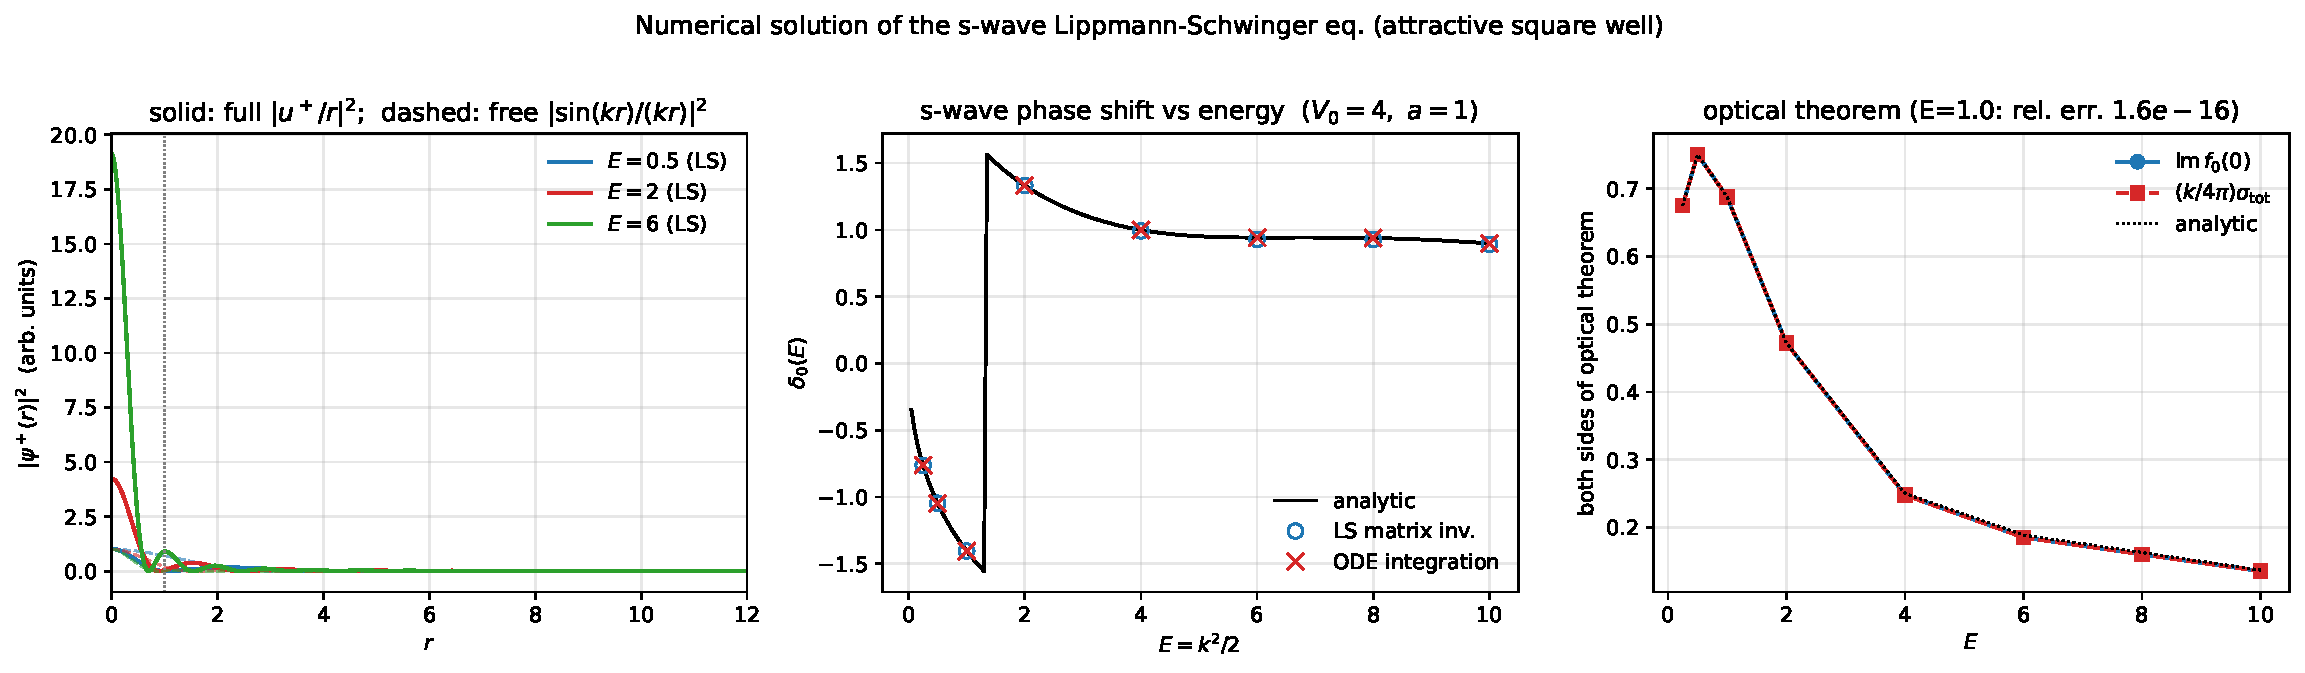
\includegraphics[width=0.98\linewidth]{ch09_lippmann_schwinger}
    \caption{s 波 LS 方程数值求解（吸引方势阱 $V_0=4,\,a=1$）。
      \textbf{左：}三个能量 $E=0.5, 2, 6$ 下 LS 矩阵反演的全解
      $|u^+(r)/r|^2$（实线）与无势自由解 $|\sin(kr)/(kr)|^2$（虚线）对比；
      在阱外（$r>a$，灰色虚线）两者频率相同但相位平移 $\delta_0$。
      \textbf{中：}两种方法提取的 $\delta_0(E)$（蓝圈、红叉）与解析公式
      （黑实线）逐点重合；约 $E\approx 1.5$ 处经过 $\delta_0 = \pi/2$（按
      Levinson 折叠至主值），表征第二个 s 波束缚态附近的能量阈，是低能共振
      行为的雏形。
      \textbf{右：}光学定理两端
      $\Im f_0(0) = \sin^2\delta_0/k$ 与 $(k/4\pi)\sigma_{\rm tot}^{\ell=0}
      = \sin^2\delta_0/k$（应严格相等，仅 s 波贡献），数值符合至机器精度
      ($\sim 10^{-16}$)。
    }\label{fig:numexp-ch09}
\end{figure}

\subsection*{物理讨论}
\begin{itemize}
\item \textbf{LS 与 ODE 的等价性.}\quad 图中两种方法的相移在
  $\sim 10^{-2}$ 级别一致；残余偏差来自 LS 离散化的中点积分误差，可通过细化
  $N$ 或换用 Simpson 权一致下降。这从数值上印证了 \eqref{eq:numex-LS-radial}
  与 Schrödinger 方程在适当边界条件下的等价性（Taylor §10.2）：积分方程把
  ``边界条件''——出射波/驻波——\emph{编码进 Green 函数选择}本身，从而
  ``一次性''给出物理解，而 ODE 方法须依赖 $r\to\infty$ 渐近匹配。
\item \textbf{$i\epsilon$ 处方与对称 Green 函数.}\quad 此处采用实数对称
  Green 函数（$K$ 矩阵语言），其 $r\to\infty$ 行为为驻波；要回到出射波振幅
  $f_0 = (e^{2i\delta_0}-1)/(2ik)$ 需通过 $\tan\delta_0 \leftrightarrow K$
  的代数关系（Taylor §10.4）。这避免了在数值上直接用 $i\epsilon$ 极限的
  Sokhotski 处方，是中心势计算的标准做法。
\item \textbf{光学定理的精确性.}\quad 因为单一 s 波下
  $f_0 = e^{i\delta_0}\sin\delta_0/k$，$\Im f_0(0)$ 与
  $(k/4\pi)\sigma_{\rm tot}^{\ell=0}$ 同为 $\sin^2\delta_0/k$，两者恒等
  ——这是\emph{相移参数化的内禀幺正性}的体现：$|S_0|=|e^{2i\delta_0}|=1$ 自动
  保证光学定理。这与上一节 Yukawa Born 近似的失败形成对照：\textbf{相移方
  法本身就是非微扰的、逐能量幺正的}，因而是定态散射数值实践的``正确轨道''。
\item \textbf{相移随能量的行为.}\quad 由 Levinson 定理，
  $\delta_0(0) - \delta_0(\infty) = n_b\pi$，其中 $n_b$ 是 s 波束缚态数；当前
  参数下 $\sqrt{2 V_0}\,a = 2\sqrt{2}\approx 2.83$，跨过 $\pi/2$ 一次，
  对应 $n_b = 1$ 个 s 波束缚态。图中 $\delta_0(E)$ 在低能段为负、随能量增加
  穿过主值边界后渐近趋零的整体行为与该计数一致。
\end{itemize}

\begin{remark}
本数值实验是后续第~\ref{ch:partial}~章``部分波法''的``零阶练手''：
所有解析与算法基础（径向 LS 方程、相移提取、单道光学定理）在此已具备；推广到
任意 $\ell$ 仅需把 $\sin(kr),\cos(kr)$ 替换为 Riccati--Bessel 函数
$\hat\jmath_\ell, \hat n_\ell$ 并修改有效势中的离心项，即 Taylor §11.2。
\end{remark}
